\documentclass[11pt, a4paper, oneside]{book}
\usepackage[utf8]{inputenc}
\usepackage{graphicx}
\usepackage{geometry}
\usepackage{titlesec}   
\usepackage{anyfontsize}
\usepackage{lipsum}
\usepackage{amsmath}
\usepackage[colorlinks=true, allcolors=blue]{hyperref}
\usepackage{float}

    %Margen
    \geometry{
        left=3cm,
        right=3cm,
        top=3cm,
        bottom=3cm,
    }

% títulos

\titleformat{\chapter}[display]
{\normalfont\bfseries\centering}
{\vspace*{-4cm}}{0pt}{\Huge}

\begin{document}

\begin{titlepage}
    \centering
    
    % Línea S1
    \rule{\textwidth}{1.5pt}\\[0.5cm]
    
    % Título principal
    \textsc{\Huge Reporte de Documentación del}\\[0.3cm]
\textsc{\Huge Proyecto Trueque Verde}\\[0.8cm]

    
    
    % Línea s2
    \rule{\textwidth}{1.5pt}\\[1cm]
    
    % Area académica
    \large INSTITUTO TECNOLOGICO DE MATAMOROS \\[0.5cm]
    Ingenieria en Sistemas computacionales\\[1cm]

    
    % Logo de la institución (guardar como 'iitk_logo.png' en el proyecto)
    \IfFileExists{Pictures/iitk_logo.png}{
        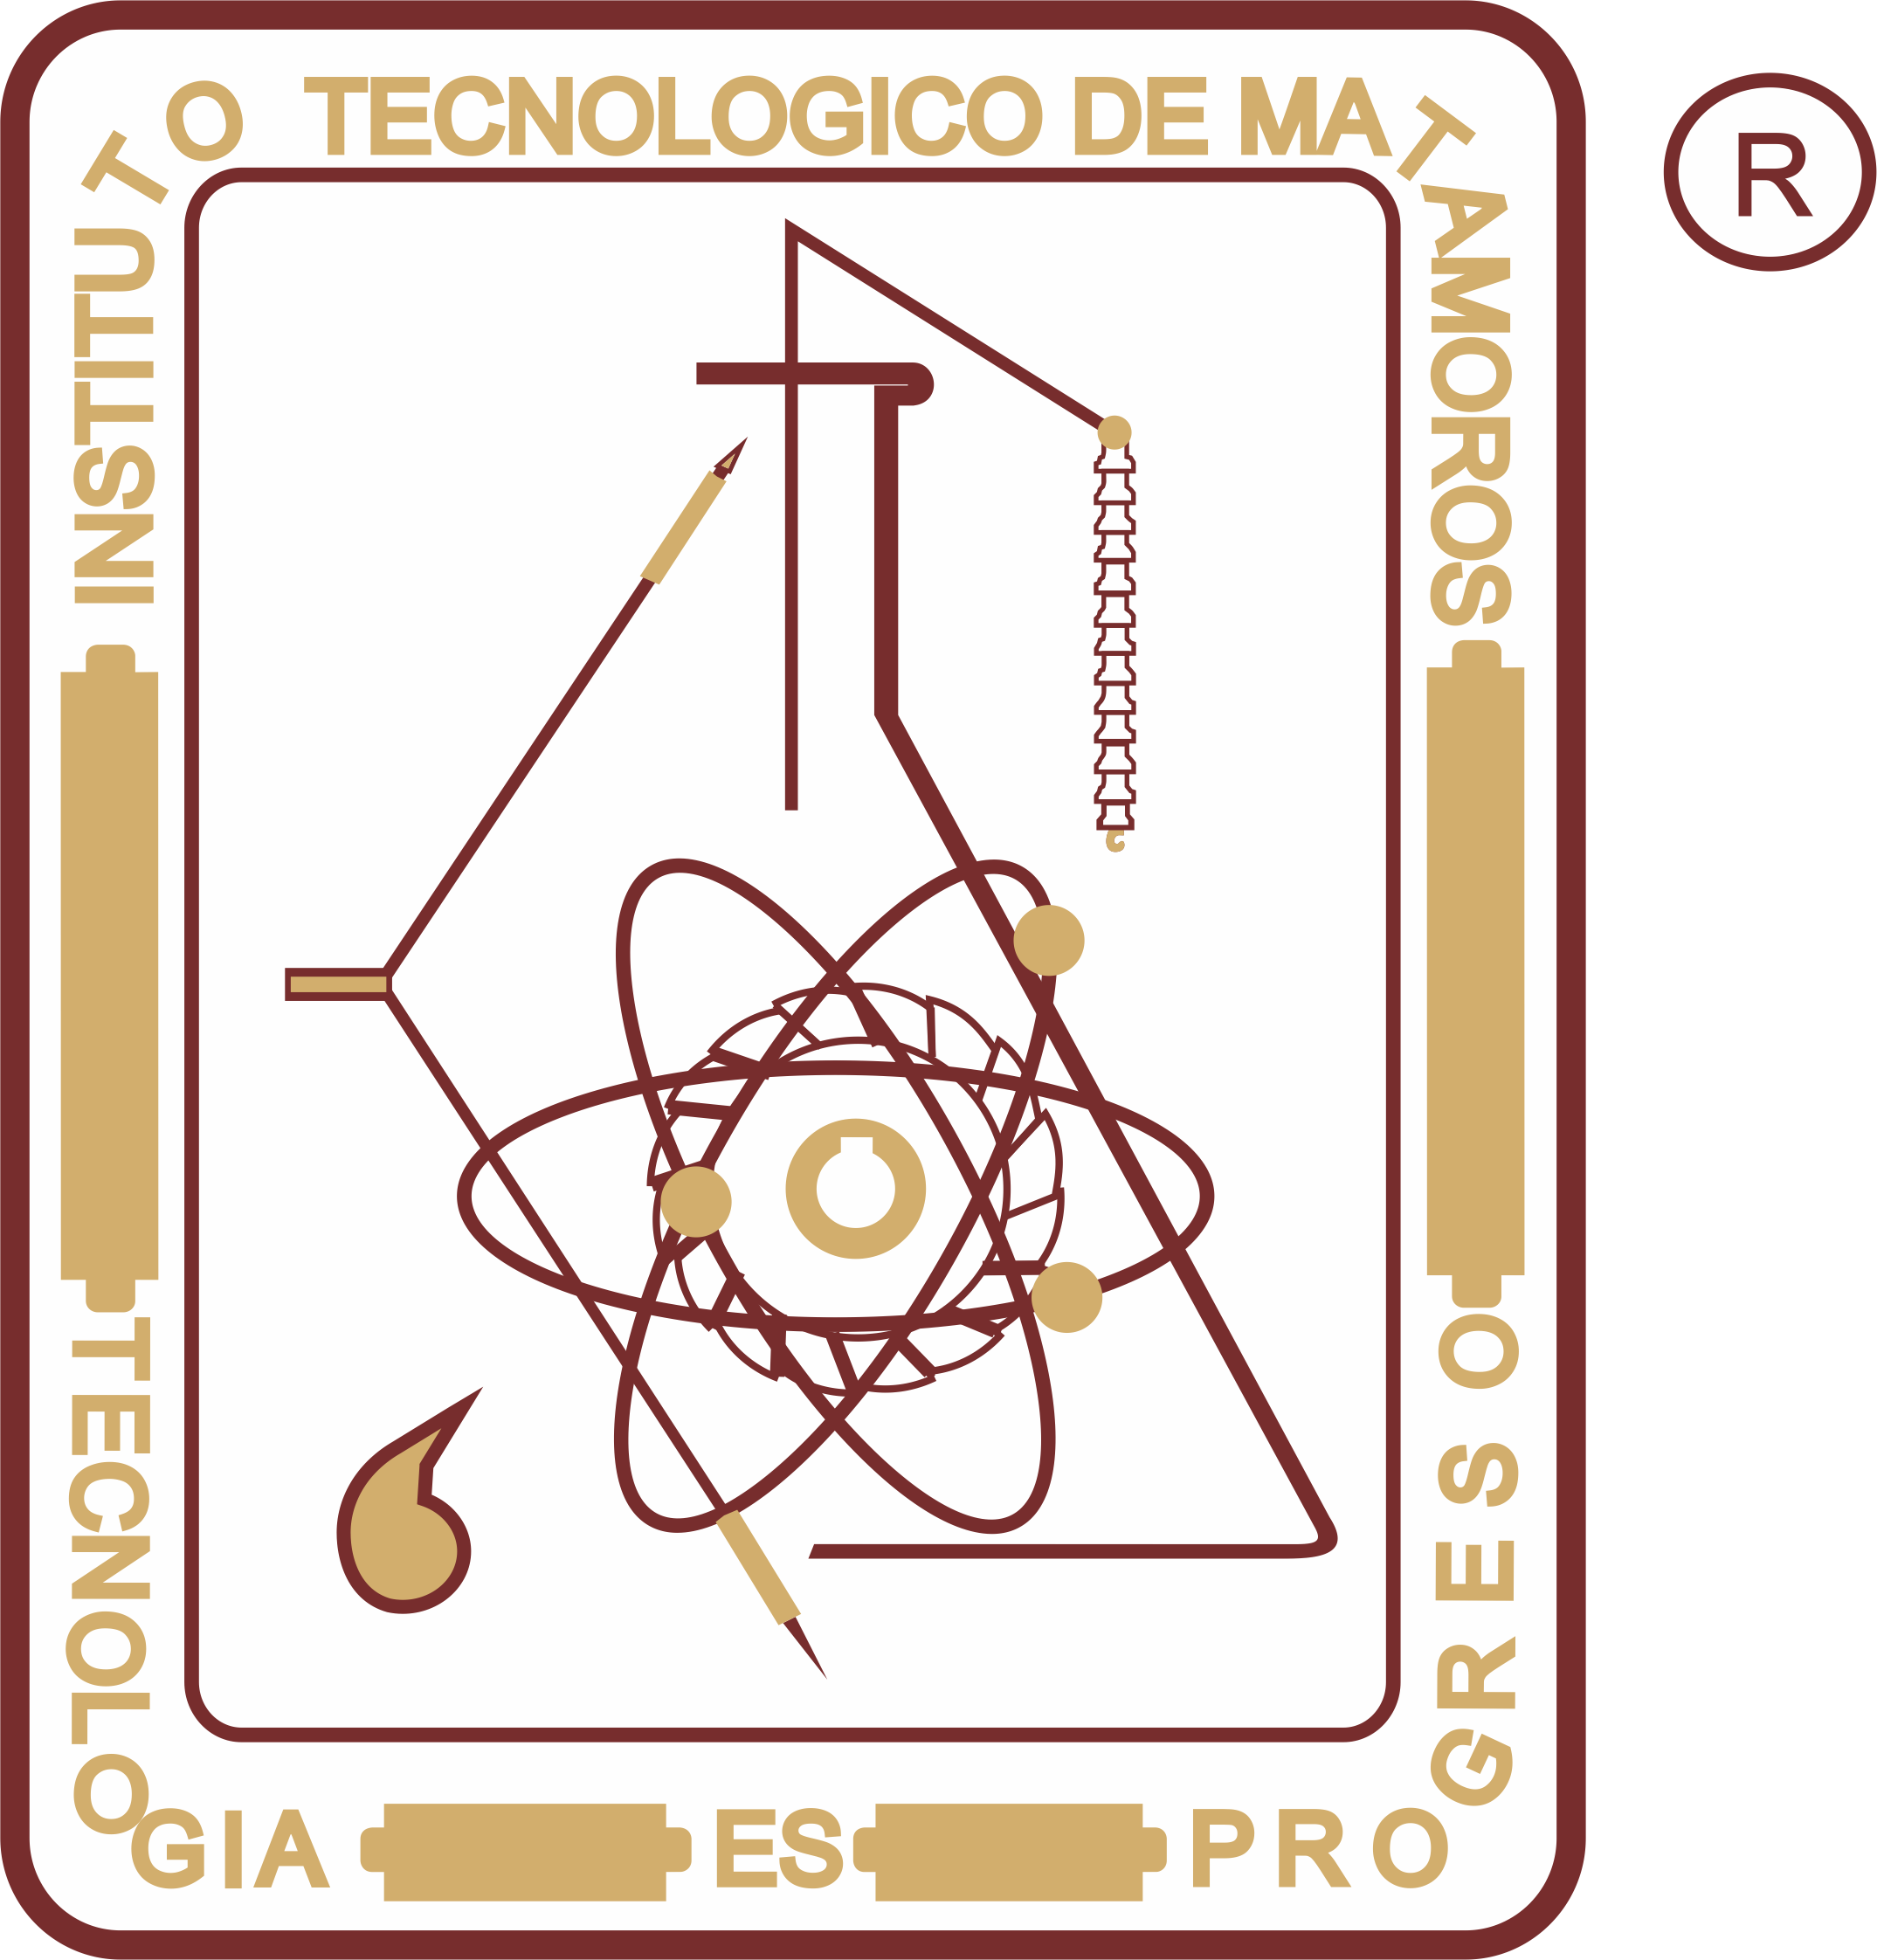
\includegraphics[width=0.3\textwidth]{Pictures/iitk_logo.png}
    }{\vspace{1.5cm}}
    \\[0.5cm]
        \textsc{Programacion FrontEnd}\\[0.5cm]

        \Large\textbf{AUTORES }\\[0.5cm]
    
    % Nombre del autor
      {\large 
      \begin{tabular}{c}
        Marcos Ivan Jimenez de la Cruz 21260170\\[0.3cm]
        Denes Ulises Mireles Rodriguez 21261105\\[0.3cm]
        Daniela Juan Hipolito 21260145\\[0.3cm]
        Esmeralda Teodoro Soreano 20260223\\[0.3cm]
        Juan Felipe Avalos Huerta 21260130\\[0.3cm]
        Ernesto Vazquez Ramirez 21260181\\
      \end{tabular}
    \par}
    \vspace{1cm}
    
    % Información institucional
    \textsc{Docente}\\[0.2cm]
    \large Anabel Pineda Briseño  \\[1cm]        
    % Fecha
    \large Marzo 2025
    
\end{titlepage}
\renewcommand{\contentsname}{Índice} 

\titleformat{\chapter}[display]
{\bfseries\centering}
{\Large Capítulo \thechapter}
{0pt}                     
{\Huge}



\titlespacing{\chapter}{0pt}{0em}{3em}


% Tabla de contenido
\tableofcontents
\newpage

% Formato del título de los capítulos
\titleformat{\chapter}[display]
{\bfseries\centering}
{%
  \\[2ex]     
  \Large Capítulo \thechapter
}
{0pt}
{\Huge}
[\vspace{3ex}]

% Ajuste de espacio entre capítulos
\titlespacing{\chapter}{0pt}{0em}{3em}

\chapter{Introducción}

\noindent El proyecto Trueque Verde surge con la finalidad de fomentar el intercambio de bienes y servicios de manera sostenible, promoviendo una economía colaborativa que incentive el cuidado del medio ambiente. En un contexto donde la responsabilidad social y el compromiso ecológico cobran cada vez más relevancia, esta plataforma se plantea como una solución integral para conectar a usuarios interesados en el intercambio responsable, facilitando tanto la comunicación como la gestión de transacciones de forma segura y amigable.

El desarrollo del proyecto se ha dividido en diversas áreas de trabajo, en las que cada equipo se ha encargado de implementar componentes específicos. Entre ellos se destacan la creación de interfaces de registro, catálogos de productos, sistemas de mensajería y mapas interactivos, tanto para plataformas web como móviles. En este sentido, el equipo 8 ha asumido la responsabilidad de recopilar y documentar de manera uniforme todos los aportes referentes al FrontEnd, con el objetivo de garantizar coherencia, facilidad de uso y mantenimiento a futuro.

Este reporte de documentación tiene como propósito describir detalladamente la estructura, diseño y funcionalidades implementadas en el FrontEnd de Trueque Verde. A través de esta guía, se busca proporcionar una visión clara y precisa de los lineamientos adoptados, los retos enfrentados y las soluciones propuestas durante el desarrollo. Además, se pretende servir como herramienta de referencia para futuros procesos de evaluación y mejora del sistema, contribuyendo al fortalecimiento de la plataforma como un recurso innovador y escalable en el ámbito del intercambio sostenible.

%Esmeralda PARTE EQUIPO 2

\chapter{Implementación de la interfaz de registro}

En este capítulo, se presentan los principales lineamientos y estrategias empleadas en el desarrollo de la interfaz de usuario, abordando desde la estructura de las vistas hasta los principios de diseño que rigen la plataforma. Se detallan aspectos clave como la disposición de los elementos en la pantalla de inicio de sesión, la organización del formulario de registro y las técnicas utilizadas para lograr una experiencia de usuario óptima.


A través de esta documentación, se proporciona una visión clara del enfoque adoptado en la construcción del FrontEnd, con el objetivo de asegurar coherencia visual, facilidad de uso y escalabilidad futura.

 
\section{Vista de Inicio de Sesión }
 La primera vista analizada corresponde a la
 pantalla de inicio de sesión, que sirve como
 punto de entrada principal para los usuarios
 registrados en la plataforma.

\begin{figure}[H]
    \centering
    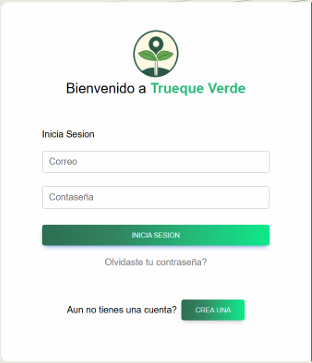
\includegraphics[width=0.55
    \linewidth]{Pictures/Bienvenido.png }
        \caption{Imagen del acceso a Git}

\end{figure}


\section{Elementos de Interfaz de Sesión } 
\begin{table}[h]
    \centering
    \renewcommand{\arraystretch}{1.5} 
    \begin{tabular}{|l|l|}
        \hline
        \textbf{Elemento} & \textbf{Texto mostrado} \\ 
        \hline
        Título principal & \textit{"Bienvenido a Trueque Verde"} \\ 
        \hline
        Etiqueta & \textit{"Inicia Sesifón"} \\ 
        \hline
        Caja de texto (input) & \textit{"Correo"} (\textit{Se introducirá el correo electrónico}) \\ 
        \hline
        Caja de texto (input) & \textit{"Contraseña"} (\textit{Se introducirá la contraseña}) \\ 
        \hline
        Botón & Iniciar sesión a la plataforma \\ 
        \hline
        Enlaces adicionales & \textit{"¿Olvidaste tu contraseña?"} y \textit{"¿Aún no tienes una cuenta?"} \\ 
        \hline
        Botón & \textit{"CREA UNA"} (\textit{Para crear una cuenta}) \\ 
        \hline
    \end{tabular}
    \caption{Elementos de la interfaz de inicio de sesión}
    \label{tabla:login}
\end{table}



\section{Implementación de Tecnicas }


\begin{itemize}
\item \textbf { Estructura HTML:}  Formulario con campos de
 entrada para correo electrónico y contraseña.
\item \textbf {Estructura CSS:} Diseño limpio con paleta de colores corporativos, utilizando flexbox o grid para la disposición de elementos.
 \item \textbf { Responsividad:}  La vista está diseñada para
 adaptarse a diferentes tamaños de pantalla.

 
\end{itemize}

\section{Vista de Registro de Usuario }
 La segunda vista corresponde al formulario
 de registro de nuevos usuarios, donde se
 recopila la información necesaria para crear
 una cuenta en la plataforma.
\begin{figure}[H]
    \centering
    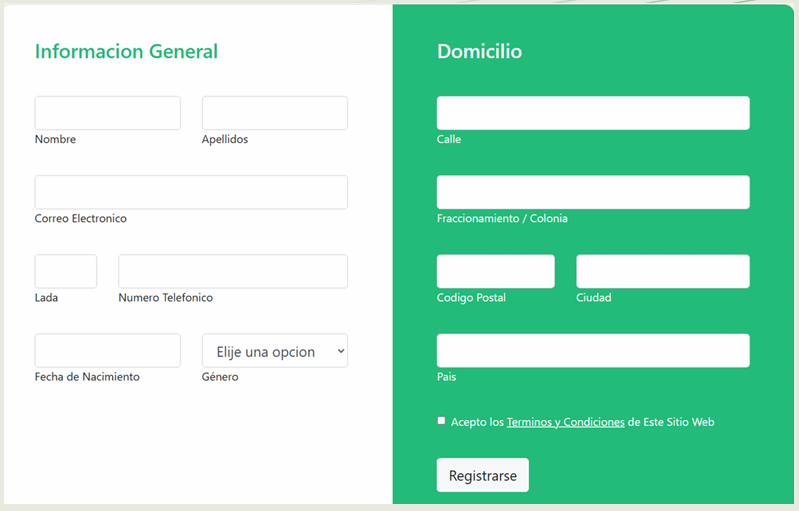
\includegraphics[width=0.7
    \linewidth]{Pictures/Sesion.png  }
            \caption{Demostración de la barra de búsqueda}
\end{figure}

\section{Elementos de interfaz}


\begin{table}[h]
    \centering
    \renewcommand{\arraystretch}{1.2}
    \small 
    \resizebox{1.1\textwidth}{!}{
    \begin{tabular}{|l|l|}
        \hline
        \textbf{Elemento} & \textbf{Descripción} \\ 
        \hline
        \textbf{Título principal} & \textit{"Información General"} \\ 
        \hline
        \textbf{Campos de información personal} & \textbf{Nombre, Apellidos, Correo Electrónico, Fecha de Nacimiento, Género} \\ 
        \hline
        \textbf{Campos de dirección} & \textbf{Calle, Fraccionamiento/Colonia, Código Postal, Ciudad, País} \\ 
        \hline
        \textbf{Campos de contacto} & \textbf{Lada, Número Telefónico} \\ 
        \hline
        \textbf{Casilla de verificación} & \textit{"Acepto los Términos y Condiciones de Este Sitio Web"} \\ 
        \hline
    \end{tabular}
    } 
    \caption{Tabla de información general}
    \label{tabla:interfaz}
\end{table}



\begin{table}[h]
    \centering
    \begin{tabular}{|l|l|}
        \hline
        \textbf{Título principal} & \textit{Información General} \\
        \hline
        \textbf{Campos de información personal} & \textbf{Nombre, Apellidos, Correo Electrónico,} \\
                                               & \textbf{\textit{Fecha de Nacimiento, Género}} \\
        \hline
        \textbf{Campos de dirección} & \textbf{Calle, Fraccionamiento/Colonia, Código Postal,} \\
                                     & \textbf{\textit{Ciudad, País}} \\
        \hline
        \textbf{Campos de contacto} & \textbf{\textit{Lada, Número Telefónico}} \\
        \hline
        \textbf{Casilla de verificación} & \textit{"Acepto los Términos y Condiciones de Este Sitio Web"} \\
        \hline
    \end{tabular}
    \caption{Tabla de información del Domicilio }
    \label{tab:info}
\end{table}

\section{Implementación de Tecnicas Utilizadas }


\begin{itemize}
\item \textbf { Estructura HTML:}   Formulario extenso con
 diversos tipos de campos de
 entrada (text, email, date,
 radio buttons, checkbox)
 
\item \textbf {Agrupación de campos:}  Los campos están
 organizados lógicamente
 por categorías
 (información personal,
 domicilio, contacto)
 
 \item \textbf { Validación de formularios:}  Implementa validación
 tanto del lado del cliente
 (HTML5/JavaScript) como
 del servidor
 
 \item \textbf {  Estilos CSS:}  Diseño de formulario
 estructurado con etiquetas
 claras y espaciado
 adecuado entre campos
 
 \end{itemize}




\section{Sistema de diseño}
Ambas vistas comparten elementos de un sistema de diseño coherente que define
 la identidad visual de Trueque Verde.

\begin{itemize}
    \item \textbf{ Paleta de colores:}  Predominancia de tonos verdes (alineados con el
 nombre "Trueque Verde") combinados con
 colores neutros para el texto y fondos. 
 
    \item \textbf{Tipografía:}  Fuente sans-serif moderna para facilitar la
 legibilidad en entornos digitales.
 
    \item \textbf{ Componentes reutilizables:}  Campos de formulario, botones y enlaces con
 estilos consistentes.
 \end{itemize}





%DENES PARTE EQUIPO 2
\chapter{Implementación del catálogo de productos de intercambio}
\noindent 
\section{Introducción}

Consideraciones técnicas:
\begin{itemize}
\item Estructura en React Native: Implementación basada en componentes reutilizables.
\item Estilos: Uso de estilos en compartidos para coherencia visual y optimización de rendimiento.
\item Navegación: Integrada con React Navigation para permitir transiciones fluidas entre vistas.
\item Categorías y colores: Implementadas mediante un mapeo que asigna un color distintivo a cada categoría.
\end{itemize}


\section{Acceso a Git}
El desarrollo de Trueque Verde se gestiona mediante un repositorio en Git, lo que permite un trabajo colaborativo eficiente, control de versiones y seguimiento de cambios en el código. A través de ramas y commits organizados, aseguramos la estabilidad del proyecto y facilitamos la integración de nuevas funcionalidades.

\begin{figure}[H]
    \centering
    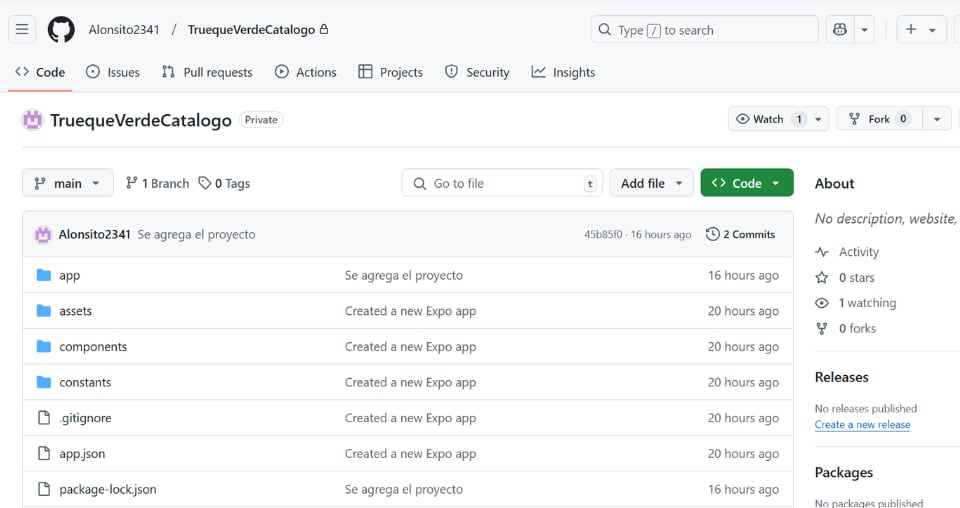
\includegraphics[width=0.80
    \linewidth]{Pictures/git.jpg}
        \caption{Imagen del acceso a Git}

\end{figure}

\section{Implementación del Catálogo de Productos de Intercambio}
Trueque Verde, una plataforma para el intercambio sostenible de productos, incluye una sección dedicada al catálogo de productos donde los usuarios podrán publicar, buscar e interactuar con productos disponibles para intercambio.
La vista principal de esta sección es el Catálogo de Productos y está diseñada para proporcionar una experiencia intuitiva, visualmente atractiva y funcional. A continuación, se detallan sus características clave:

\section{Pantalla de Catalogo}
\begin{itemize}
\item Barra de busqueda.\\
Permite a los usuarios buscar productos por nombre, categoría o descripción.
\begin{figure}[H]
    \centering
    
\includegraphics[width=0.5
    \linewidth]{Pictures/BarraBusqueda.png  }
            \caption{Demostración de la barra de búsqueda}
\end{figure}

\item Botón de filtro.\\
Permite aplicar filtros según categorías como frutas, verduras, semillas, etc.

\begin{figure}[H]
    \centering
    \begin{minipage}{0.35\linewidth}
        \centering
        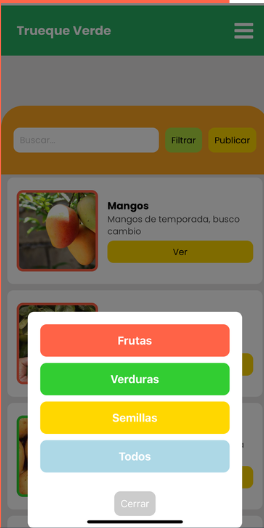
\includegraphics[width=\linewidth]{Pictures/BotonFiltro.png}
        \caption{Demostración de los posibles
filtros a seleccionar.}
    \end{minipage}
    \hfill
    \begin{minipage}{0.40\linewidth}
        \centering
        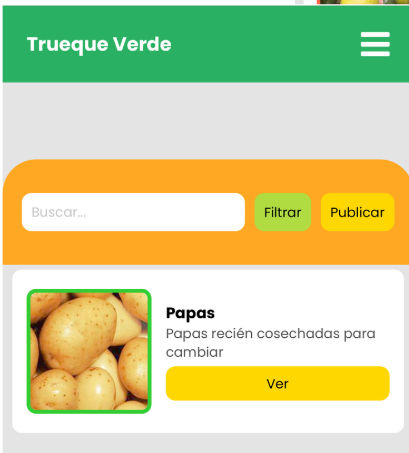
\includegraphics[width=\linewidth]{Pictures/BotonFiltroDemostracion.png}
        \caption{Imagen con los filtros aplicados.}
    \end{minipage}
\end{figure}

\item Botón de publicar.\\
Los usuarios pueden agregar nuevos productos para intercambio mediante un formulario.

\begin{figure}[H]
    \centering
    
\includegraphics[width=0.45
    \linewidth]{Pictures/BotonPublicar.png  }
            \caption{Demostración del botón publicar}
\end{figure}

\item Listado de productos.\\
Se muestran en un formato de tarjeta con una imagen, nombre, descripción y un botón para ver más detalles.

\begin{figure}[H]
    \centering
    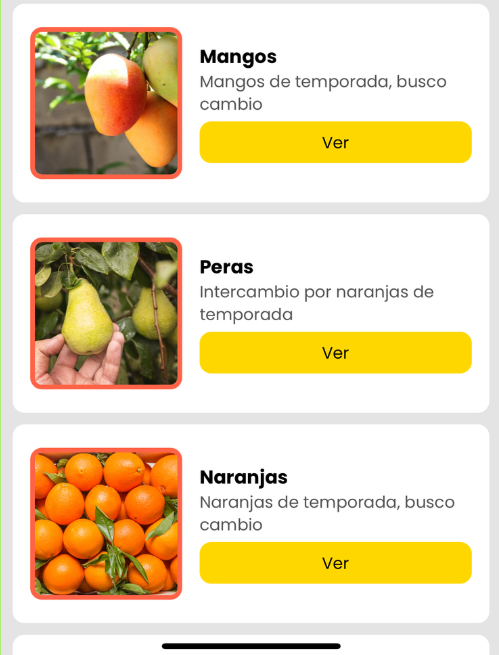
\includegraphics[width=0.5
    \linewidth]{Pictures/ListaProductos.png  }
            \caption{Demostración del listado de productos}
\end{figure}

\end{itemize}


\section{Pantalla del Producto}
Al seleccionar un producto en el catálogo, los usuarios acceden a la pantalla de detalles, donde pueden obtener información más específica sobre el producto seleccionado.
\subsection{Titulo principal}
Nombre del producto con fondo de color según su categoría.

\begin{figure}[H]
    \centering
    
\includegraphics[width=0.5
    \linewidth]{Pictures/TituloProducto.png  }
            \caption{Titulo del producto seleccionado}
\end{figure}

\subsection{Imagen del producto}
Se utiliza un carrusel de imágenes del producto.

\begin{figure}[H]
    \centering
    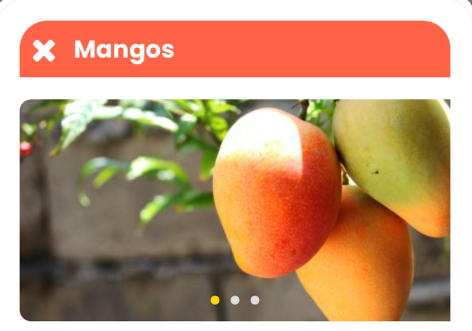
\includegraphics[width=0.5
    \linewidth]{Pictures/ImagenProducto.png  }
            \caption{imagen del producto seleccionado}
\end{figure}

\subsection{Contactar al usuario}
Chat con el usuario para contactarlo y realizar el intercambio.

\begin{figure}[H]
    \centering
    
\includegraphics[width=0.75
    \linewidth]{Pictures/ContactarUsuario.png  }
            \caption{Sección donde se contactara al dueño del producto.}
\end{figure}

\subsection{Descripción completa}
Explicación detallada del producto y sus características.

\begin{figure}[H]
    \centering
    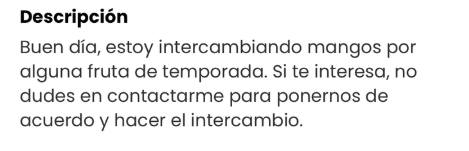
\includegraphics[width=0.60
    \linewidth]{Pictures/DescripcionProducto.png  }
            \caption{Demostración de la descripción del producto}
\end{figure}

\subsection{Información del usuario}
Calificación de intercambios del usuario.

\begin{figure}[H]
    \centering
    
\includegraphics[width=0.75
    \linewidth]{Pictures/InformacionUsuario.png  }
            \caption{ Demostración de la información del usuario}
\end{figure}

\subsection{Ubicación del producto}
Indica dónde se encuentra disponible para el intercambio.

\begin{figure}[H]
    \centering
    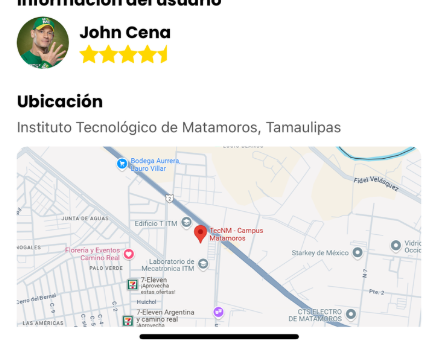
\includegraphics[width=0.75
    \linewidth]{Pictures/UbicacionUsuario.png  }
            \caption{ Mapa de demostraci´on donde el usuario puede hacer encuentros de intercambio.}
\end{figure}
%DANIELA EQUIPO 3_
\chapter{Implementación del sistema de intercambio}
\noindent


\section{Formulario y Chat}

\subsection{Funcionalidades Principales}
     las funcionalidades mencionadas:
     
\begin{itemize}
    \item Chat integrado: Permite a los usuarios ponerse de acuerdo fácilmente.
\end{itemize}

\begin{itemize}
    \item Formulario de intercambio: Ayuda a registrar qué se ofrece, qué se busca a cambio, la ubicación y hasta agregar fotos.
\end{itemize}

\begin{itemize}
    \item Diseño sencillo e intuitivo: La aplicación está pensada para que cualquiera pueda usarla sin problemas.
\end{itemize}

\subsection{Estructura}
     Pantallas Principales:
\begin{itemize}
    \item Pantalla de inicio para explorar opciones de trueque 
\end{itemize}


\begin{itemize}
    \item Pantalla del chat para negociar intercambios 
\end{itemize}

\begin{figure}[H]
\centering
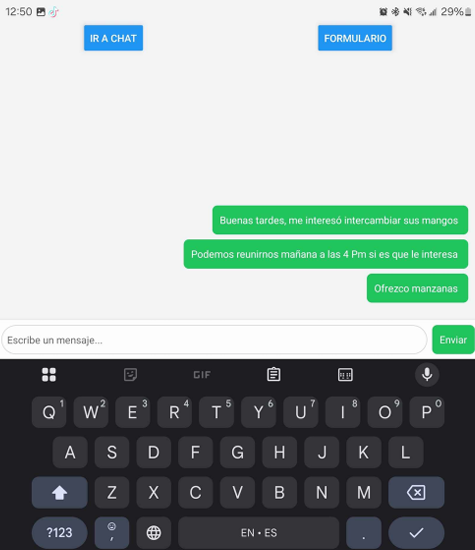
\includegraphics[width=0.4\textwidth]{Pictures/chat.png}
\caption{Chat}
\end{figure}

\begin{itemize}
    \item Formulario de Intercambios  
\end{itemize}

\begin{figure}[H]
\centering
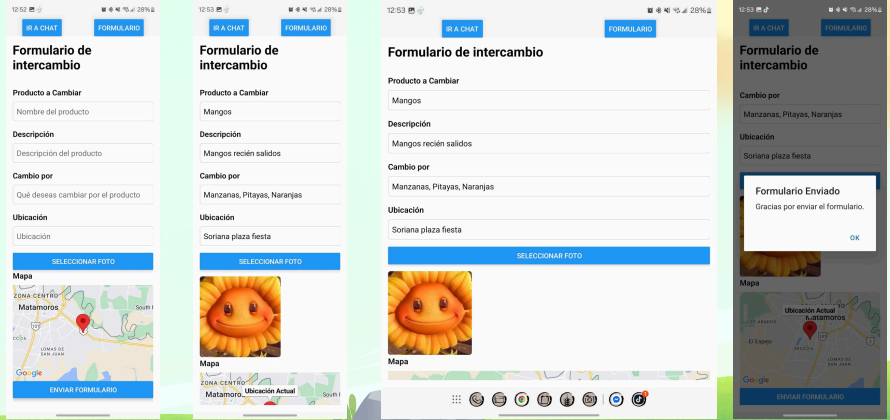
\includegraphics[width=1\textwidth]{Pictures/trueque.png}
\caption{Formulario}
\end{figure}

\begin{itemize}
    \item Archivo Principal: App.tsx, donde se organiza el funcionamiento basico de la App 
\end{itemize}


\chapter{Implementacion de Mapa Interactivo }

Entre las principales funcionalidades de la aplicación se encuentra un mapa interactivo que permite a los usuarios visualizar las zonas donde hay personas dispuestas a intercambiar productos. También cuenta con puntos de intercambio comunitarios, que son lugares recomendados para llevar a cabo los trueques de manera segura.


Para el desarrollo de la aplicación móvil se utilizó React Native, apoyado en Expo para facilitar la configuración y el despliegue. Además, se implementó un backend en Laravel con una API REST que permite la comunicación entre la aplicación y la base de datos mediante Axios. La configuración del proyecto se realizó con Expo CLI, y su estructura principal incluye archivos clave como package.json (para dependencias), app.json (configuración de Expo) y App.js (punto de entrada de la aplicación)

\section{Pruebas en Dispositivos}
En cuanto a las pruebas, se utilizó Expo Go para ejecutar el proyecto en dispositivos móviles en tiempo real, asegurando la comunicación con el backend mediante la IP local del equipo de desarrollo.
\begin{figure}[H]
\centering
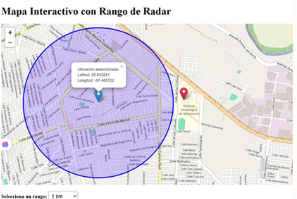
\includegraphics[width=0.8\textwidth]{Pictures/mapa.png}
\caption{Referencia del Radio de comunicación}
\end{figure}

\begin{figure}[H]
\centering
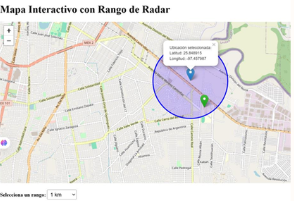
\includegraphics[width=0.8\textwidth]{Pictures/mapa2.png}
\caption{Imagen con Vista mas amplia}

\end{figure}
\begin{figure}[H]
\centering
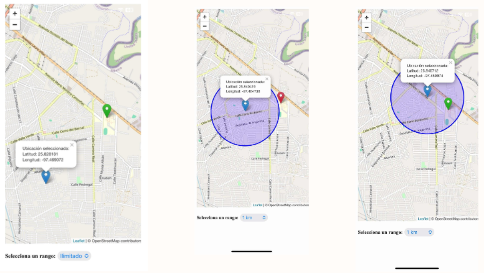
\includegraphics[width=0.8\textwidth]{Pictures/mapa3.png}
\caption{Imagen referencial en movil}
\end{figure}

Durante el proceso, se presentaron algunos problemas, como la obsolescencia de Expo CLI, errores con la configuración del Android SDK y la no detección del punto de entrada de la aplicación en Expo. Estos inconvenientes fueron solucionados mediante la actualización de herramientas, la correcta configuración de variables del entorno y la limpieza de caché para forzar la recarga de la aplicación.


\chapter{Implementación de la interfaz (Pagina Web) }
\noindent
\section{Estructura del proyecto}
El proyecto \textbf{\textbf{"Educación Verde"}} es una página web diseñada para educar a los usuarios sobre el cuidado de árboles frutales. La página incluye secciones con consejos, guías, beneficios y características de diferentes árboles frutales. Además, utiliza Bootstrap para el diseño responsivo y JavaScript para generar contenido dinámico el proyecto está compuesto por los siguientes archivos:

\textbf{\subsection {index.html}}
Archivo principal que contiene la estructura HTML de la página.

\textbf{1}  \textbf{\textbf{Encabezado (<header>)}}:

    Contiene el logo y el título de la página.
    
    Diseño responsivo con Bootstrap.

\textbf{2}  \textbf{\textbf{Contenido Principal (<main>)}}:

Secciones para \textbf{\textbf{Consejos}}, \textbf{\textbf{Guías}}, \textbf{\textbf{Beneficios}} y \textbf{\textbf{Árboles Frutales}}.

Cada sección utiliza un contenedor dinámico (<div id="consejos-container">, etc.) 

que se llena con JavaScript.

\textbf{3}  \textbf{\textbf{Pie de Página (<footer>)}}:

Información de derechos de autor y enlaces a políticas de privacidad y contacto.

\textbf{4}  \textbf{\textbf{Modal}}:

Un modal de Bootstrap que muestra información adicional al hacer clic en los 

botones "Leer más".


\subsection{ styles.css}
Archivo de estilos CSS personalizados.

\textbf{1 }  \textbf{\textbf{Estilos Generales}}:

 Fuente predeterminada: Arial, sans-serif.

 Fondo de la página: \#f8f9fa.

\textbf{2}  \textbf{\textbf{Estilos para el Header}}:

 Fondo verde (\#28a745) con texto blanco.

Logo redondeado y sombra.

\textbf{3}  \textbf{\textbf{Estilos para las Cards}}:

 Efecto hover que levanta la card y agrega sombra.

Imágenes con altura fija y bordes redondeados.

\textbf{4}\textbf{  \textbf{Estilos para el Footer}}:

 Fondo oscuro (\#343a40) con texto blanco.

Enlaces con efecto hover que cambian de color.


\subsection{script.js}

\textbf{1}  \textbf{\textbf{Arrays de Datos}}:

consejos, guias, beneficios, arbolesFrutales: Arrays que contienen la información 

que se muestra en las secciones.

\textbf{2 }  \textbf{\textbf{Funciones Principales}}:

generarConsejos(), generarGuias(), generarBeneficios(), generarArbolesFrutales(): 

Generan el contenido dinámico para cada sección.

mostrarDetalles(), mostrarDetallesGuias(), mostrarDetallesBeneficios(), 

mostrarCaracteristicas(), mostrarCuidados(), mostrarPlantado(): Muestran 

información detallada en el modal.

\textbf{3 }  \textbf{\textbf{Event Listener}}:

 DOMContentLoaded: Ejecuta las funciones de generación de contenido cuando la 
 
 página se carga.



\section{Funcionalidades}

\subsection {Sección de consejos}
Muestra una lista de consejos para cuidar árboles frutales.
Cada consejo incluye una imagen, un título, una descripción breve y un botón "Leer más" que abre un modal con detalles adicionales.
\begin{figure}[H]
\centering
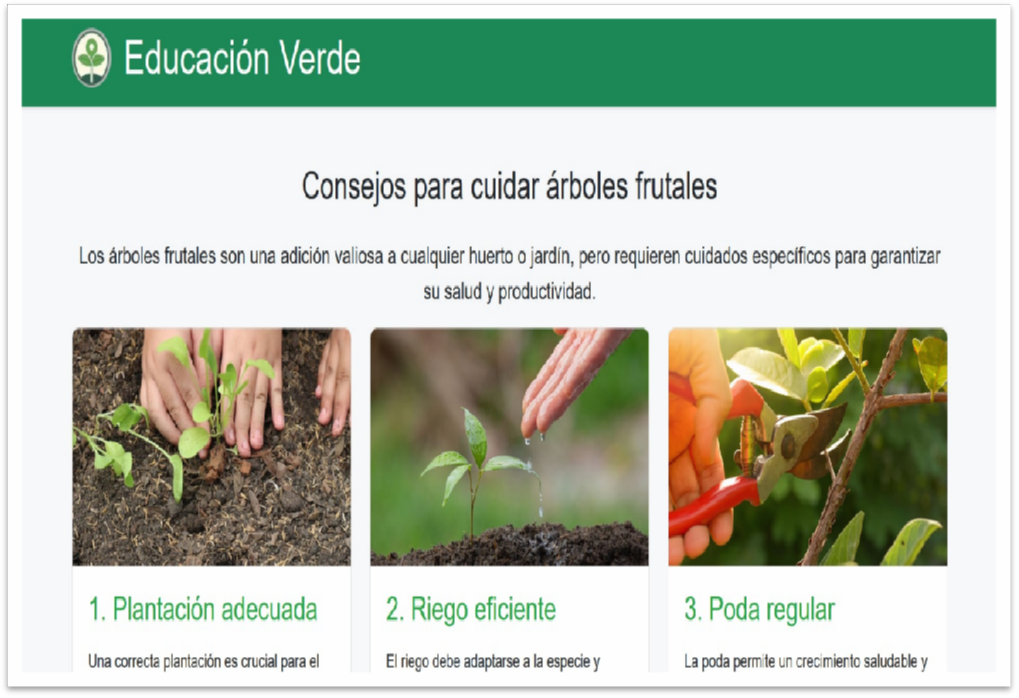
\includegraphics[width=0.9\textwidth]{Pictures/consejos.png}
\caption{Imagen de Consejos}
\end{figure}
\subsection {Sección de guías}
Proporciona guías prácticas para plantar y mantener árboles jóvenes.
Similar a la sección de consejos, incluye imágenes, títulos, descripciones y un botón para ver más detalles.
\begin{figure}[H]
\centering
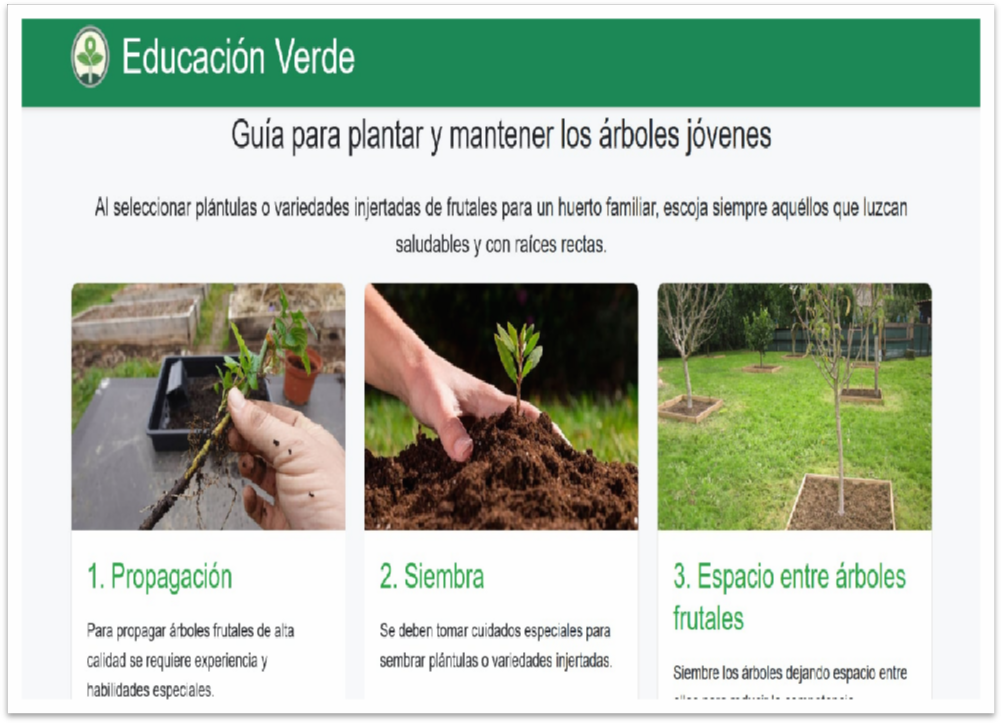
\includegraphics[width=0.75\textwidth]{Pictures/guias.png}
\caption{Referencia del Radio de comunicación}
\end{figure}
\subsection { Sección de beneficios}
Enumera los beneficios de los árboles frutales para el medio ambiente.
Cada beneficio tiene una imagen y un botón para ver más información en el modal.
\begin{figure}[H]
\centering
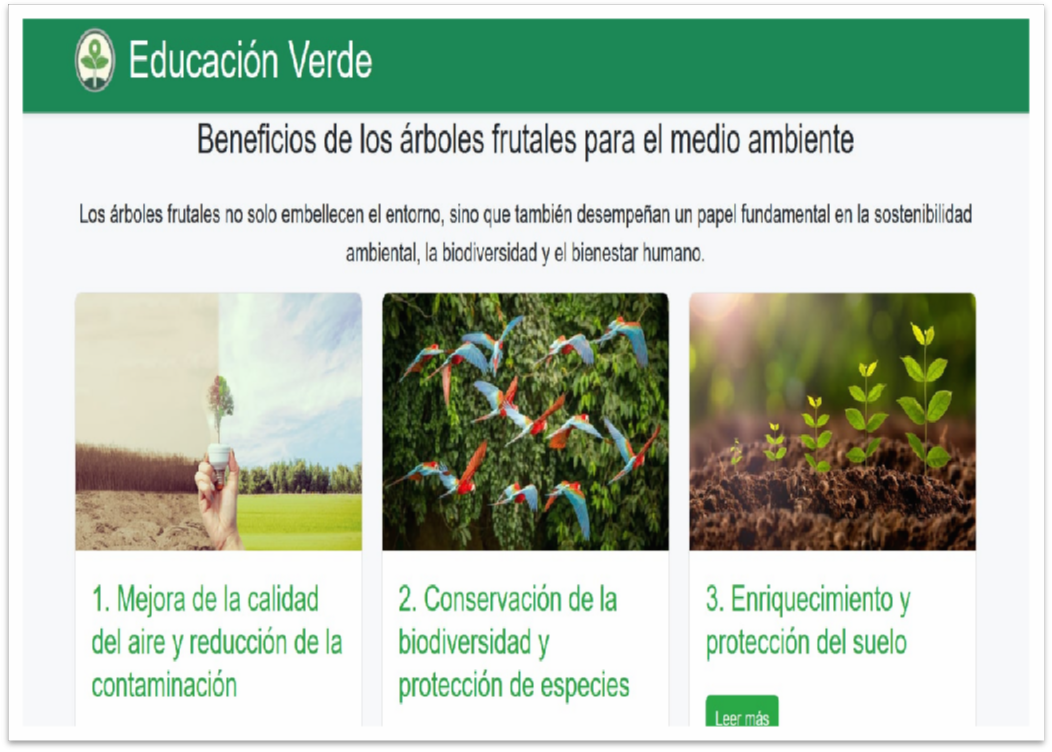
\includegraphics[width=0.75\textwidth]{Pictures/beneficios.png}
\caption{Referencia del Radio de comunicación}
\end{figure}
\subsection {Sección de árboles frutales}
Presenta una lista de árboles frutales con sus características, cuidados y recomendaciones de plantación.
\begin{figure}[H]
\centering
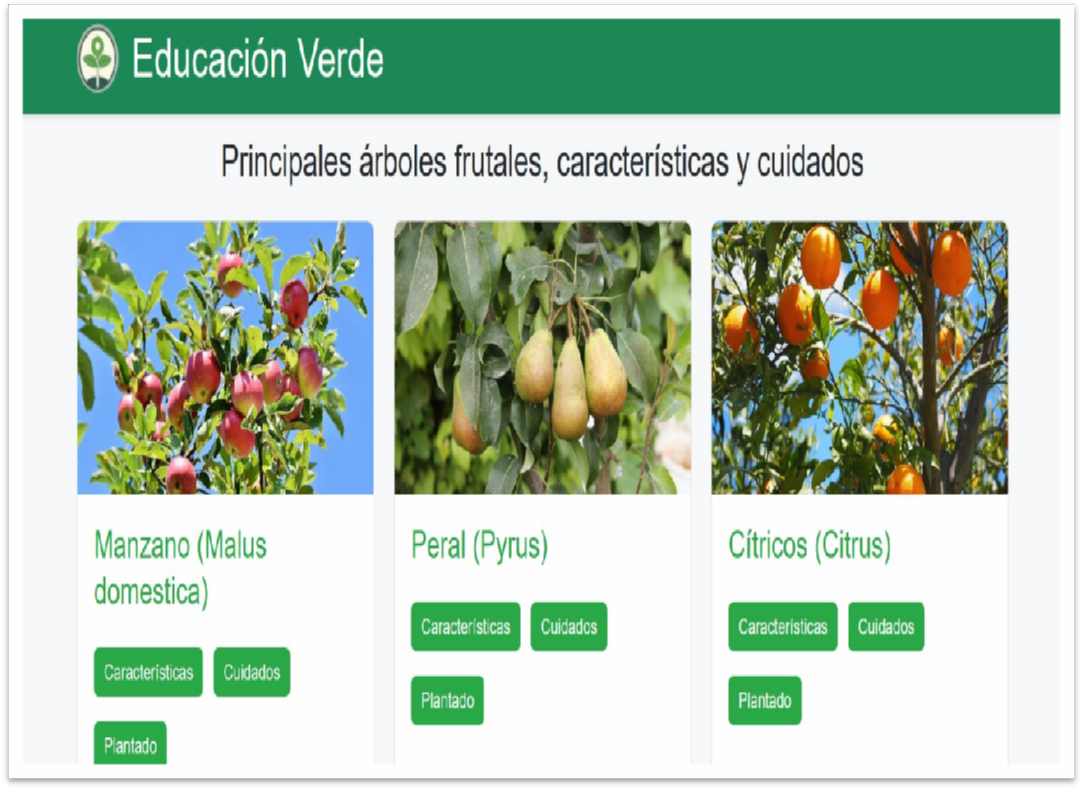
\includegraphics[width=0.8\textwidth]{Pictures/arboles.png}
\caption{Referencia del Radio de comunicación}
\end{figure}

Cada árbol tiene tres botones para ver detalles sobre sus características, cuidados y cómo plantarlo.

\subsection {Modal}
Un modal reutilizable que muestra información detallada dependiendo del botón que se haya hecho clic.
\begin{figure}[H]
\centering
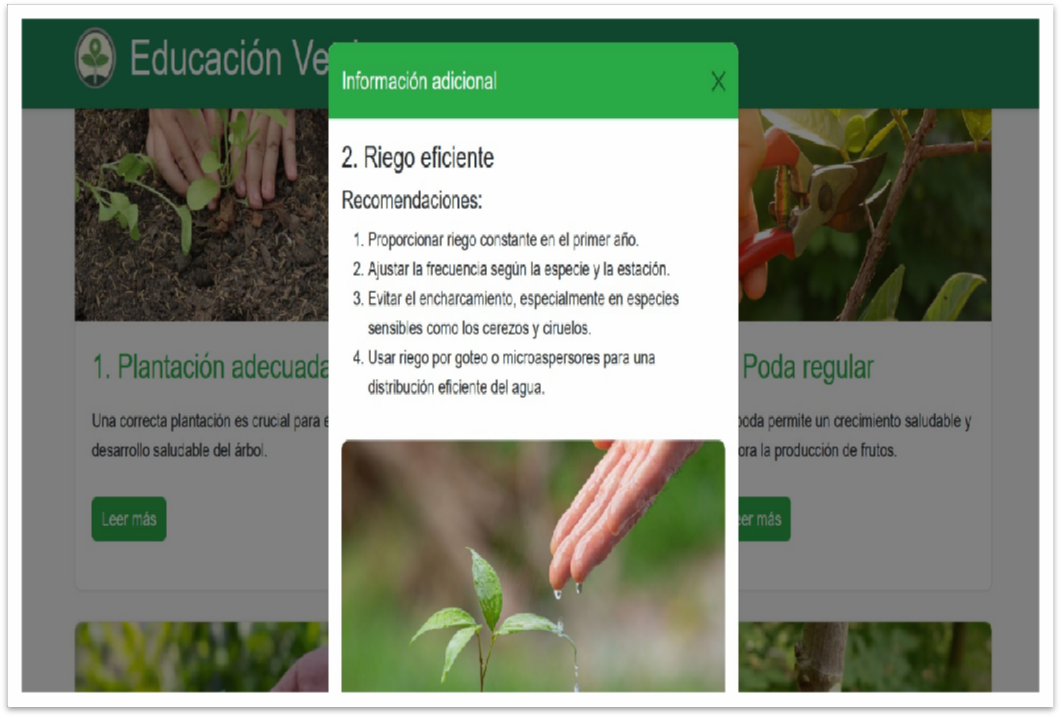
\includegraphics[width=0.6\textwidth]{Pictures/modal.png}
\caption{Referencia del Radio de comunicación}
\end{figure}

El contenido del modal se genera dinámicamente con JavaScript.



\chapter{Implementación de la interfaz Sistema de Reputacion (móvil)} 

La implementación de la interfaz móvil en Trueque Verde es un componente esencial para la evaluación y el despliegue de reputación de los participantes. Para lograr una experiencia intuitiva y funcional, se han utilizado herramientas como React Native y Nativewind, permitiendo un diseño dinámico y adaptable a distintos dispositivos.
\hspace{2cm}

El desarrollo se centra en la construcción de una interfaz clara y accesible, donde los usuarios podrán visualizar su nivel de reputación, gestionar productos disponibles e interactuar con otros participantes a través de un menú desplegable.


\section{Herramientas}

•	Visual Studio Code

•	Nativewing

•	Github

•	Javascript

•	React Native

•	CSS



\section{Elementos de la Interfaz}

•	Menú Desplegable

•	Nombre del Usuario

•	Nivel de Reputación

•	Imagen del Usuario

•	Rango del Usuario

•	Productos Disponible

\hspace{0cm}

\hspace{2cm}

\hspace{4cm}

\section{Encuesta de Satisfacción del Cliente}

\begin{figure}[H]
    \centering
    \begin{minipage}{0.3\textwidth} 
        \centering
        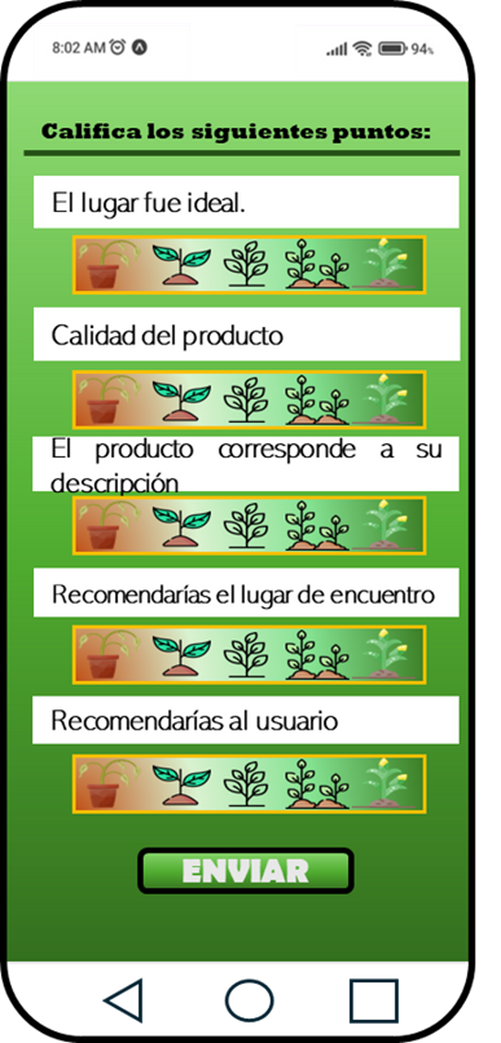
\includegraphics[width=\textwidth]{Pictures/Imagen 1.png}
        \caption{Imagen de selección}
    \end{minipage}
    \hfill 
    \begin{minipage}{0.3\textwidth}
        \centering
        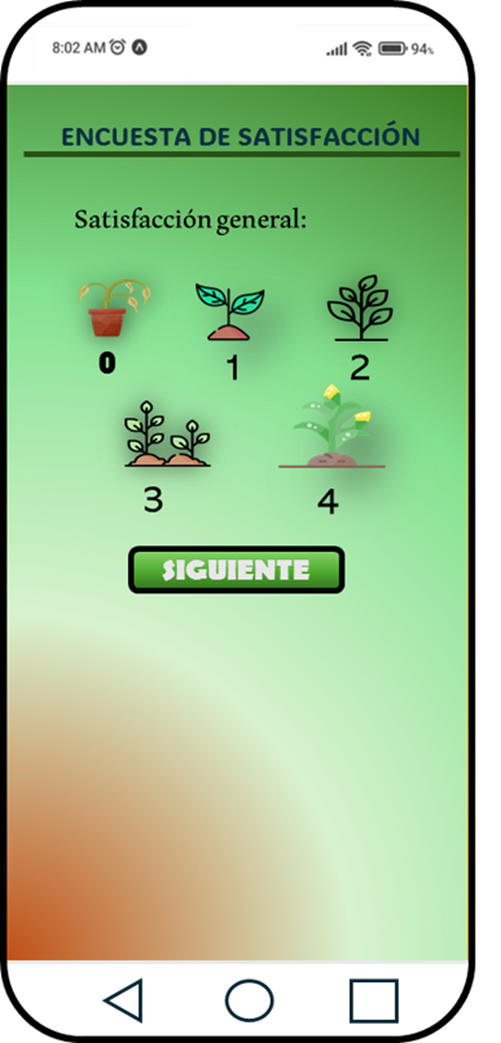
\includegraphics[width=\textwidth]{Pictures/Imagen 2.png}
        \caption{imagen de satisfaccion 2}
    \end{minipage}
    \hfill
    \begin{minipage}{0.3\textwidth}
        \centering
        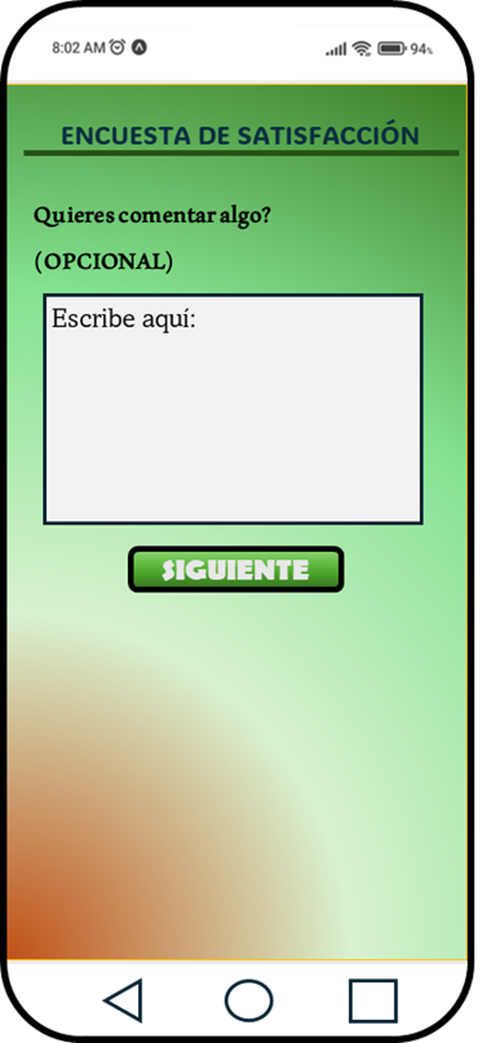
\includegraphics[width=\textwidth]{Pictures/Imagen 3.png}
        \caption{aEncuesta Mensaje}
    \end{minipage}
\end{figure}

\chapter{ Implementación de la interfaz del panel de administración }

El sistema de moderación de usuarios y publicaciones está diseñado para garantizar un entorno seguro dentro de la plataforma. Para ello, se han implementado funcionalidades que permiten la gestión de reportes, la revisión de publicaciones y la toma de decisiones sobre su estado.

\hspace{2cm}

Para optimizar el proceso de moderación, se han incorporado ventanas emergentes (modales) que muestran información detallada de cada reporte, incluyendo la fecha, el motivo y el usuario denunciante, además de opciones para tomar medidas directamente desde la interfaz.

\section{Usuarios Problemáticos }

Listado de Características y Funcionalidades del código,búsqueda de reportes tabla de usuarios responsable.


• Usuario reportado.

• Razón del reporte (ejemplo: "Contenido ofensivo").

• Cantidad de reportes recibidos.

• Estado del usuario. 

\hspace{6cm}

\section{Publicaciones } 

Este código implementa una página de administración para la moderación de publicaciones reportadas dentro de una plataforma. Su propósito es permitir que los
administradores revisen, aprueben o eliminen publicaciones que han sido reportadas por los usuarios. 



1-Filtros para Buscar Publicaciones Reportadas



• Pendiente de revisión" → No ha sido moderada aún. 


• "Eliminada" → Se consideró inadecuada y se borró.


• "Aprobada" → Se validó y es visible para los usuarios.


• Botón "Filtrar" para aplicar los criterios de búsqueda.

\section{Tabla de Publicaciones } 


• ID único de la publicación.

• Usuario que realizó la publicación.

• Razón del reporte (ejemplo: "Contenido ofensivo").

Estado actual de la publicación:

• Pendiente de revisión → Necesita ser moderada.

• Eliminada → Se eliminó por incumplimiento de normas.

• Aprobada con advertencia → Permitida, pero el usuario fue advertido.

Acciones disponibles para cada publicación:

• "Ver Detalles" → Muestra información completa de la publicación en un modal.

• "Advertir" → Envía una advertencia al usuario sobre su contenido.

• "Eliminar" → Elimina la publicación por incumplir normas.

• "Aprobar" → Permite que la publicación se mantenga visible. 

\section{Ventanas Emergentes (Modales) con Detalles de la Publicación} 

Usuario 1 tiene un modal con información detallada:

• Fecha del reporte: 21-02-2025.

• Razón: Contenido ofensivo.

• Reportado por: @usuarioReportadorX.

Contenido de la publicación:

• Imagen publicada (placeholder de imagen).

• Texto de la publicación, visible en un bloque de cita.

Acciones disponibles dentro del modal:

• Advertir al usuario sobre el contenido.

• Eliminar la publicación si infringe normas.

• Aprobar la publicación si no hay problemas.

\chapter{Equipos de Trabajos}

\section*{Equipo 1}
\begin{itemize}
    \item Isaac Segovia Cazares
    \item Johan Adrian Gonzalez Loza
    \item Felipe Jesus Hernandez Guzman
    \item Mauricio Eliseo Rosales Weigend
    \item Kevin del Angel Colunga Vazquez
    \item Santiago Emmanuel Garcia Villanueva
\end{itemize}

\section*{Equipo 2}
\begin{itemize}
    \item Camarillo Estrada Alonso Emmanuel
    \item González Rodríguez Kevin Eduardo
    \item Jiménez Reséndiz Karla Rebeca
    \item Muñoz Ordoñez José Daniel
\end{itemize}

\section*{Equipo 3}
\begin{itemize}
    \item Alcocer Rangel Fernando
    \item Del Angel Díaz Danniel Ehud
    \item López Nava Alejandro
    \item Lozano Velazquez Brandon Armando
    \item Torres Martínez José Francisco
    \item Ramos González Edgar Karol
\end{itemize}

\section*{Equipo 4}
\begin{itemize}
    \item Jan Karlo Armendariz Gonzalez
    \item Leslie Yiharem Aguirre Isassi
    \item Andrea Sordel Guzmán
    \item Jessica Rubi Gallegos Rodriguez
    \item Joel Sánchez Gutiérrez
    \item Fabiola de Jesus Cuellar Hiyan
\end{itemize}

\section*{Equipo 5}
\begin{itemize}
    \item Garibaldi Zúñiga, Daniel
    \item González Pérez, Erick Eduardo
    \item Herrera Galaviz, Leonardo
    \item Márquez Ruiz, José de Jesús
    \item Rivera Jaramillo, Jesús Naum
\end{itemize}

\section*{Equipo 6}
\begin{itemize}
    \item Padron Zaleta Jared Alfredo
    \item Patiño Herrera Edgar Ivan
    \item Perez Calderon Gerardo Adrian
    \item Lopez Cantu Andres Manuel
    \item Zaleta Diaz Dalia Nohemi
    \item Gutierrez Mendoza Osbel Emmanuel
\end{itemize}

\end{document}

\end{document}
